\documentclass[a4paper,11pt]{article}
\usepackage[utf8]{inputenc}
\usepackage[francais]{babel}
\usepackage[T1]{fontenc}

\usepackage[toc,page]{appendix}
%fonts pour les math
\usepackage{amsfonts}
\usepackage{amsmath}
\usepackage{dsfont}
%couleur dans le doc
\usepackage[dvipsnames]{xcolor}

\usepackage{enumitem}
\frenchbsetup{StandardLists=true}
\usepackage{multirow}
\usepackage{hyperref}

%affichage lignes de code
\usepackage{listings}
\usepackage{textcomp}
\lstset{
	tabsize=2,
	language=python,
        basicstyle=\scriptsize,
        upquote=true,
        aboveskip={0.2\baselineskip},
        columns=fixed,
        showstringspaces=false,
        extendedchars=true,
        breaklines=true,
        prebreak = \raisebox{0ex}[0ex][0ex]{\ensuremath{\hookleftarrow}},
        frame=single,
        showtabs=false,
        showspaces=false,
        showstringspaces=false,
        identifierstyle=\ttfamily,
        keywordstyle=\color[rgb]{0,0,1},
        commentstyle=\color[rgb]{0.133,0.545,0.133},
        stringstyle=\color[rgb]{0.627,0.126,0.941},
}

%\usepackage{lastpage}
%pour les images
	\usepackage[dvips, pdftex]{graphicx}
	\usepackage[section]{placeins}
	\usepackage{here}	
	\usepackage{float}

%définition du titre du document
 \newcommand{\titleinfo}{INF441-NET - NetProbes} 

%formattage de la page
	\usepackage{geometry}
	\geometry{top=2cm, bottom=2cm, left=2cm, right=2cm}
	%fomattage de l'entête et du pied de page
	\usepackage{fancyhdr}
	\pagestyle{fancy}
		\setlength{\headheight}{15.2pt}
		\lhead{\titleinfo\\}
		\rhead{\leftmark}
	%Page de garde avec style vide
	\thispagestyle{empty}	
	

%formattage du titre des sections
	%\usepackage{titlesec}
	%\titleformat{\section}[runin]{\normalfont\bfseries}{\sectionprefix \thesection}{1pt}{}[.]

%longueur des sauts de paragraphe
\setlength{\parskip}{1ex}

%commande pour les ensembles
\newcommand{\R}{\mathbb{R}}
\newcommand{\N}{\mathbb{N}}
\newcommand{\C}{\mathbb{C}}
\newcommand{\cd}[1]{\texttt{#1}}

%commande pour les notations de map
	%\newcommand{\I}{\mathds{1}}
	%\newcommand{\p}{\mathds{P}}
	%\newcommand{\E}{\mathds{E}}
	%\renewcommand{\P}{\mathds{P}}


%commande pour les opérateurs
\newcommand{\INT}{\displaystyle\int}
\newcommand{\SUM}{\displaystyle\sum}
\newcommand{\FRAC}{\displaystyle\frac}
\newcommand{\PROD}{\displaystyle\prod}
\newcommand{\INF}{\displaystyle\inf}

%commande pour environnement description
\newcommand{\desc}[1]{\item[] \texttt{#1}}
\usepackage{hyperref}
\hypersetup{
    colorlinks,
    citecolor=black,
    filecolor=black,
    linkcolor=black,
    urlcolor=black
}

\begin{document}

\thispagestyle{empty}							%page de garde vide
%\begin{document}
	\begin{center}
		\hfill
		François \bsc{Espinet}
		\hfill \hfill
		Gaspard \bsc{Ferey}
		\hfill ~
		\par
		\noindent
		\\
		\vspace{0.7cm}
		\textit{Promotion X2011}
		\vfill\vfill
		\Huge
		\begin{tabular}{c}
			\hline
			%Projet\\
			NetProbes\\
			{\Large{\textsc{~~~~~INF441-NET~~~~~}}}\\
			\hline
		\end{tabular}
		\large
		\vfill
		Diagnostics réseau distribués
	\end{center}
	\vfill
	\begin{flushright}
	
\includegraphics[scale=0.1]{img/logo_x.png}
	\end{flushright}
	\newpage 


\tableofcontents

\section{NetProbes : un programme de diagnostic réseau distribué}
Le but de ce programme est de permettre d'effectuer des tests sur un réseau donnée.

Après avoir établit un réseau de sondes par dessus le réseau test via http, on pourra lancer les tests de notre choix sur ce réseau et collecter les résultats pour analyse.

L'architecture de l'application nous permet d'implémenter des tests à la volée. En effet, il suffit de placer un module python implémentant les bonnes fonctions dans le dossier probe/tests afin que le nouveau test puisse être utilisé. Notre but a donc plus été de proposer une méthode de synchronisation autour des tests que le code des tests eux-mêmes.

\section{Guide de l'utilisateur}

\subsection{Prérequis}
\begin{description}
\item[Python3] l'interpréteur python est requis. Nous avons développé notre application pour la version 3.3.\\
Pour plus d'information sur l'installation de Python3, consulter cette page :
\begin{center}
\href{http://docs.activestate.com/activepython/3.2/diveintopython3/html/installing-python.html}{http://docs.activestate.com/activepython/3.2/diveintopython3/html/installing-python.html}
\end{center}

\item[Connexion HTTP] une connexion HTTP entre les sondes est requise afin de permettre la synchronisation autour des tests et les opération de construction du réseau de sonde.
\end{description}


\subsection{Installation}
\begin{enumerate}
\item Décompresser l'archive dans un dossier au choix.
\item Se placer en ligne de commande dans un des sous-dossier : commander ou probe.
\item Lancer l'exécutable python : main.py
\end{enumerate}
Remarque: dans les exemples sous Windows suivants, Python3 a été ajouté au path via une commande du type:
\begin{center} \texttt{ { \color{blue}C:$\backslash$...$\backslash$NetProbes$>$}path \%path\%;c:$\backslash$python33} \end{center}

\subsection{Manuel d'utilisation}

\subsubsection{Options au lancement}
Les options pour les différents programme sont donnés par l'option -h à l'invocation du main : python main.py -h.
Ceci est valable pour les deux exécutables que nous fournissons.\\
Exemple\\
Sous Windows: \ \ \ \texttt{ { \color{blue}C:$\backslash$...$\backslash$NetProbes$\backslash$app$\backslash$probe$>$}python main.py -h}

\subsubsection{Sondes : package probe}
La première étape de l'utilisation de notre outil consister à faire tourner plusieurs sonde sur différentes machines connectées à un même réseau. L'utilisation des sondes est transparente et autonome. Les commandes d'ajout/suppression et de test étant effectuées par l'interface utilisateur.

Une sonde se lance par une simple exécution du programme python \texttt{main.py}.

La sonde est par défaut verbeuse, à moins de spécifier l'option --no-debug lors de son lancement.

Il est également possible de lui spécifier un identifiant avec l'option -id.

Pour quitter la sonde, la seule solution implémentée est d'utiliser Ctrl+C sous Linux ou de fermer la console sous Windows.

Exemple sous Windows:\\
\texttt{ { \color{blue} C:$\backslash$...$\backslash$NetProbes$>$}cd app$\backslash$probe}\\
\texttt{ { \color{blue} C:$\backslash$...$\backslash$NetProbes$\backslash$app$\backslash$probe$>$}python main.py -id sondeA ---no-debug}


\subsubsection{Interface utilisateur : package commander}
L'interface permet de commander une sonde de son choix. On peut choisir l'adresse IP de cette sonde au démarrage avec l'option -ip.

Exemple sous Windows:
\begin{center}
\texttt{ { \color{blue}C:$\backslash$...$\backslash$NetProbes$\backslash$app$\backslash$commander$>$}python main.py -i gui -ip 127.0.0.1}
\end{center} 
Un fois la connexion établie, on obtient l'affichage suivant :

\begin{figure}[!ht]
\begin{minipage}[c]{0.5\linewidth}
\centering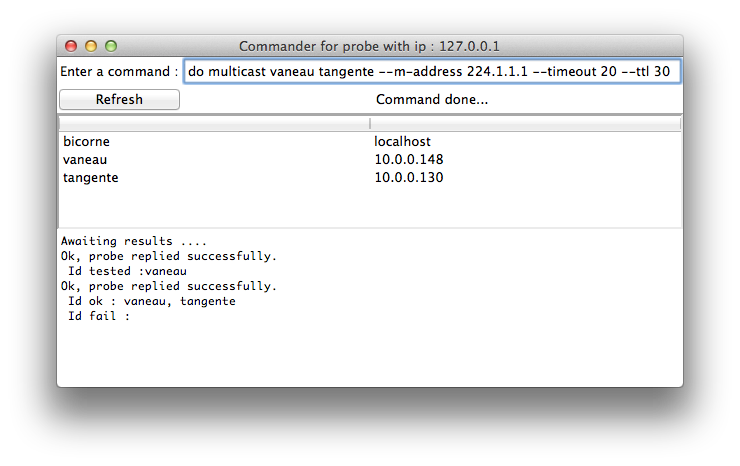
\includegraphics[width=\linewidth]{img/commander.png}
\end{minipage}
\hfill
\begin{minipage}[c]{0.5\linewidth}
\begin{description}
\item[ligne d'entrée] permet de donner des commandes à la sonde
\item[ligne de statut] permet d'afficher le status de la commande exécutée
\item[bouton rafraichir] permet de rafraichir les sondes connues en les demandant au serveur commandé
\item[affichage des sondes] tableau id | adresse IP des sondes connues
\item[panneau résultats] affiche les résultats des tests lancés
\end{description}
\end{minipage}
\end{figure}
\FloatBarrier

Les commandes supportés sont les suivantes :
\begin{description}
\item[add ip] ajoute la sonde d'adresse IP 'ip' à notre réseau de sondes. On peut ensuite effectuer des tests dessus.
\item[remove id] supprime la sonde id du réseau. Supprimer la sonde commandée permet de la retirer du réseau.
\item[do testname testoptions] effectue le test 'testname' sur la sonde commandée avec les options testoptions. Les options sont de la forme option=valeur.
\end{description}
\vspace{2ex}
\textbf{Affichage des résultats}

Les résultats sont automatiquement affichés lorsqu'ils sont disponibles sur la sonde commandée dans le panneau prévu à cet effet.


\subsection{Exemples}
% Mettre un capture d'écran avec des meilleurs noms
\subsubsection{Ajouter des sondes}
\texttt{add 10.0.0.148}\\
\indent\texttt{add 10.0.0.130}

\subsubsection{Effectuer des tests}
\texttt{do unicast r --port 5611 --protocol tcp}\\
\indent\texttt{do unicast r --timeout 2 --protocol udp}\\
\indent\texttt{do broadcast --port 7267 --timeout 3.5 }\\
\indent\texttt{do multicast vaneau tangente --port 12456 --timeout 3.4 --ttl 20 -ma 224.4.6.6}\\
\indent\texttt{do empty}

\section{Architecture et fonctionnement}


\subsection{Architecture}

On représente ci-dessous l'organisation globale des différents threads qui composent les sonde du réseau.
Les conventions de représentations sont les suivantes :
\begin{figure}[!ht]
\centering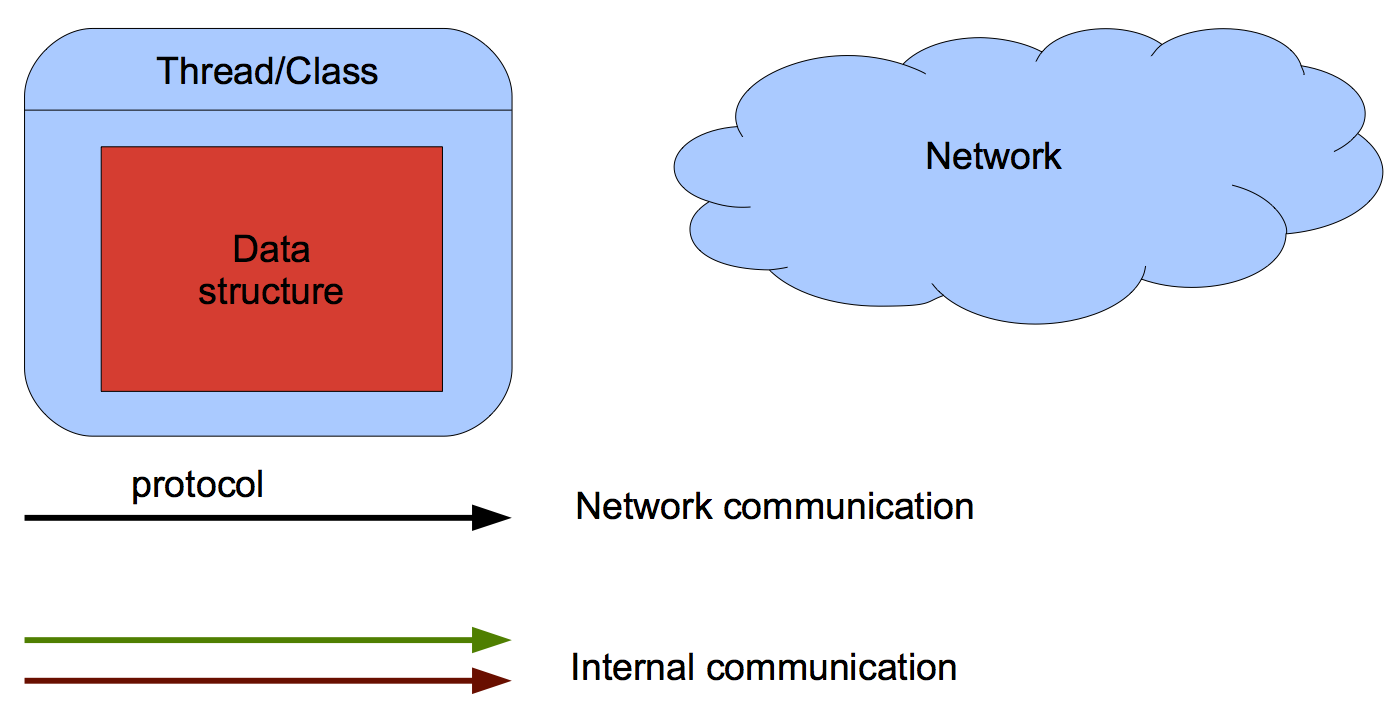
\includegraphics[width=\linewidth]{img/graphLegend.png}
\caption{Légende}
\end{figure}

\begin{figure}[!ht]
\centering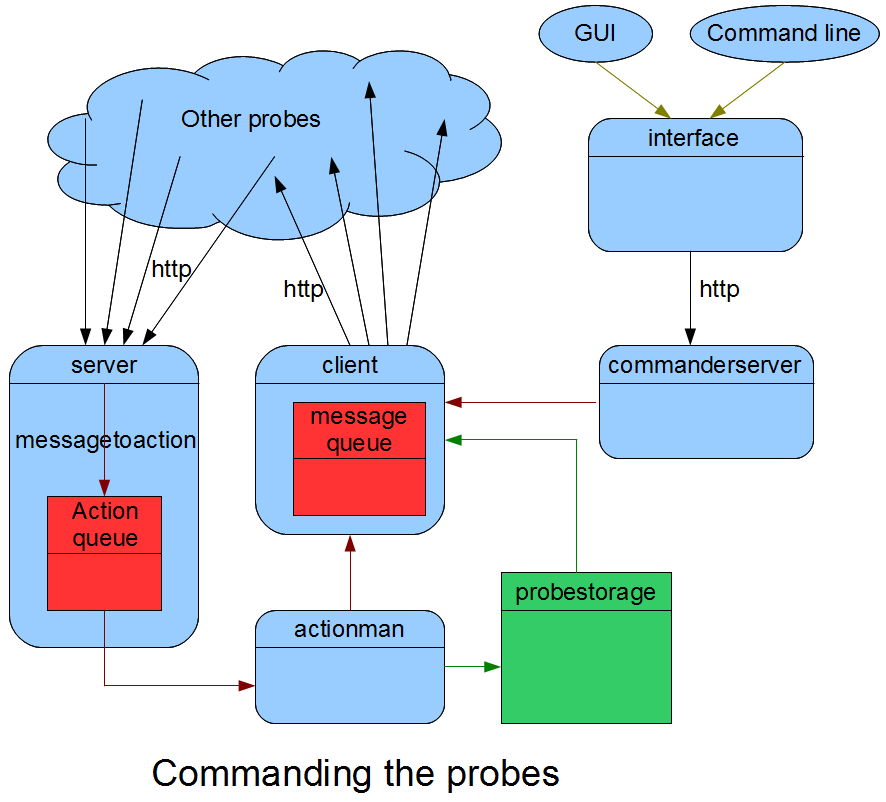
\includegraphics[width=\linewidth]{img/graphCommander.png}
\caption{Fonctionnement d'une sonde}
\end{figure}

Une sonde est composé dans sa version la plus simple de 3 threads et de 3 structures de stockage de données.
\begin{itemize}
\item L'objet \cd{ProbeStorage} contient les sondes du réseau (Id, IP), ainsi que les objets représentant les connexions HTTP vers ces sondes.
\item Le thread \cd{Client} gère une file de messages. Il utilise les connections du \cd{probestorage} pour les envoyer au fur et à mesure.
\item Le thread \cd{Server} écoute les requêtes HTTP sur le port de communication interne des sondes et transforme les messages reçu en actions qu'il stocke dans une file d'attente.
\item Le thread \cd{ActionMan} dépile les actions dans l'ordre de priorité et les exécute.
\end{itemize}
Le commander est un thread à part qui peut même être lancé à partir d'une machine sur laquelle ne tourne aucune sonde. Ce programme prend en entrée une machine (adresse IP) sur laquelle fonctionne une sonde avec qui communiquer. Il utilise cette sonde pour connaître le réseaux et déclencher des tests.
Les threads mis en jeu sont :
\begin{itemize}
\item Le thread \cd{Interface} graphique (GUI) ou en ligne de commande (CLI), elle est à la fois le serveur et le client qui permet de communiquer avec une sonde commandée.
\item Le thread \cd{CommanderServer} tourne sur la sonde et écoute les requêtes HTTP sur le port de communication "commander" des sondes. Il réagit immédiatement aux messages reçu du commander.
\end{itemize}


\begin{figure}[!ht]
\centering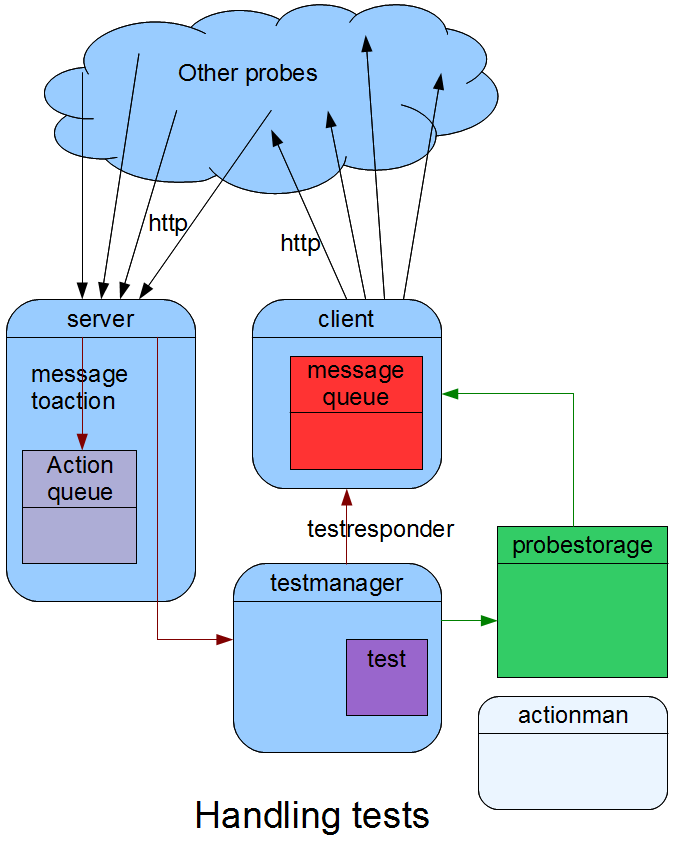
\includegraphics[width=\linewidth]{img/graphTest.png}
\caption{Fonctionnement alternatif lors d'un test}
\end{figure}

Lors de l'exécution d'un test, un thread particulier, est lancé par les sondes. Le thread \cd{ActionMan} est bloqué jusqu'à l'arrêt du test.
\begin{itemize}
\item \cd{TestManager} pour la sonde qui exécute le test.
\item \cd{TestResponder} pour les sondes qui réagissent au test.
\end{itemize}

\subsection{Fonctionnement}

\subsubsection{Ajout d'une sonde au réseau}

\begin{figure}[!ht]
\centering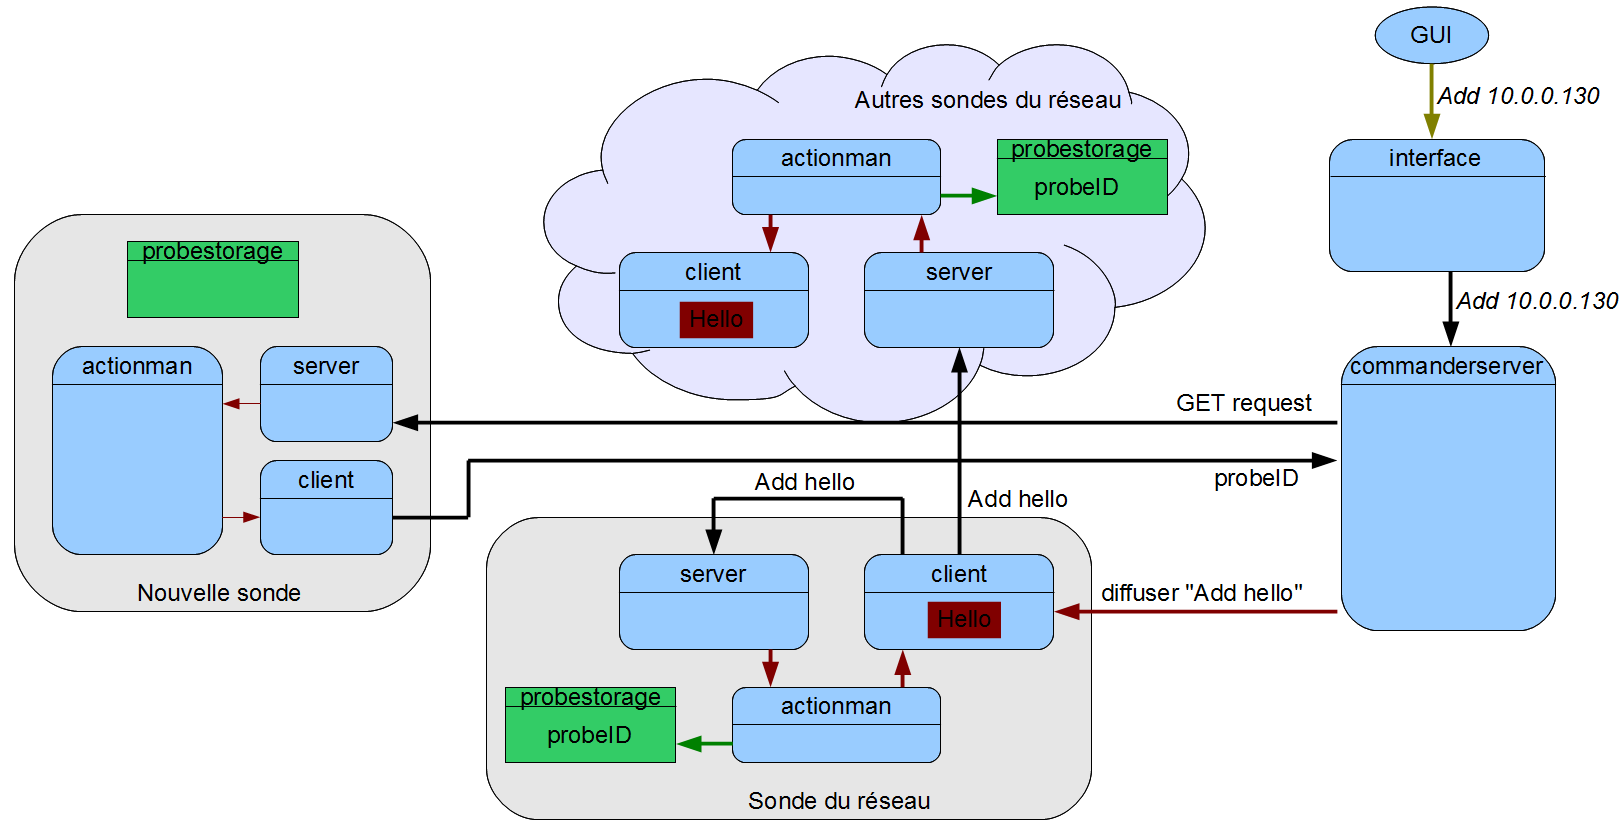
\includegraphics[width=\linewidth]{img/graphAdd1.png}
\caption{Ajout d'une sonde - Etape 1}
\end{figure}




\begin{figure}[!ht]
\centering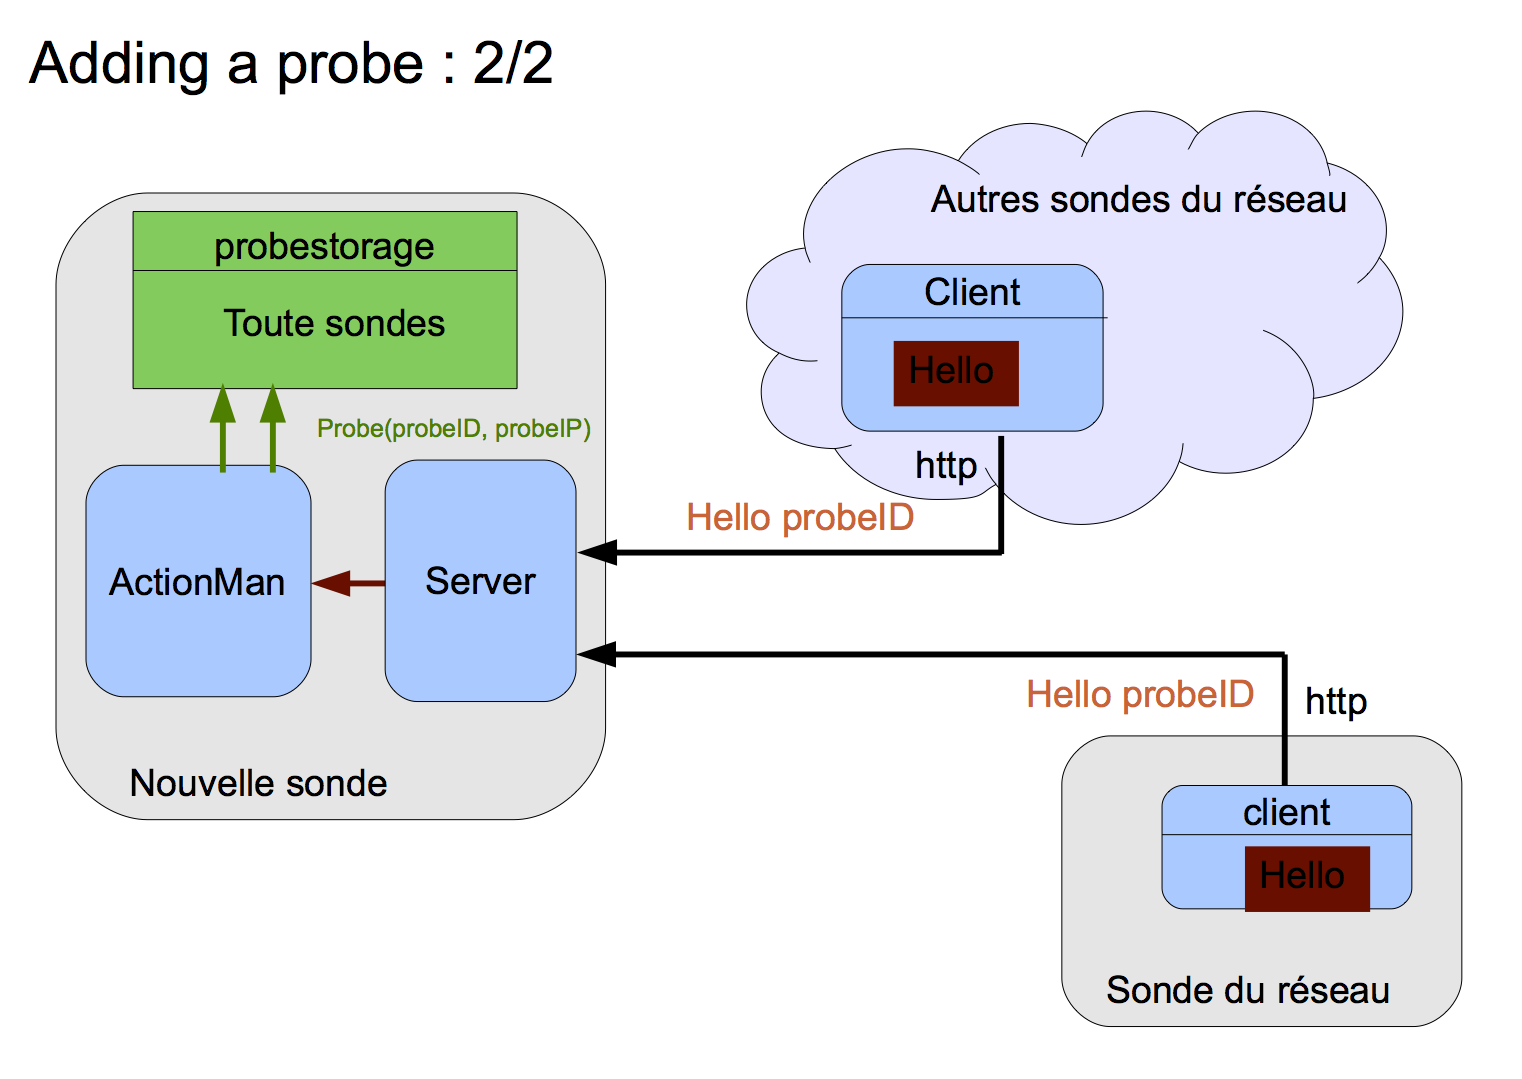
\includegraphics[width=\linewidth]{img/graphAdd2.png}
\caption{Ajout d'une sonde - Etape 2}
\end{figure}

\FloatBarrier
\subsubsection{Exécution d'un test}

\begin{figure}[!ht]
\centering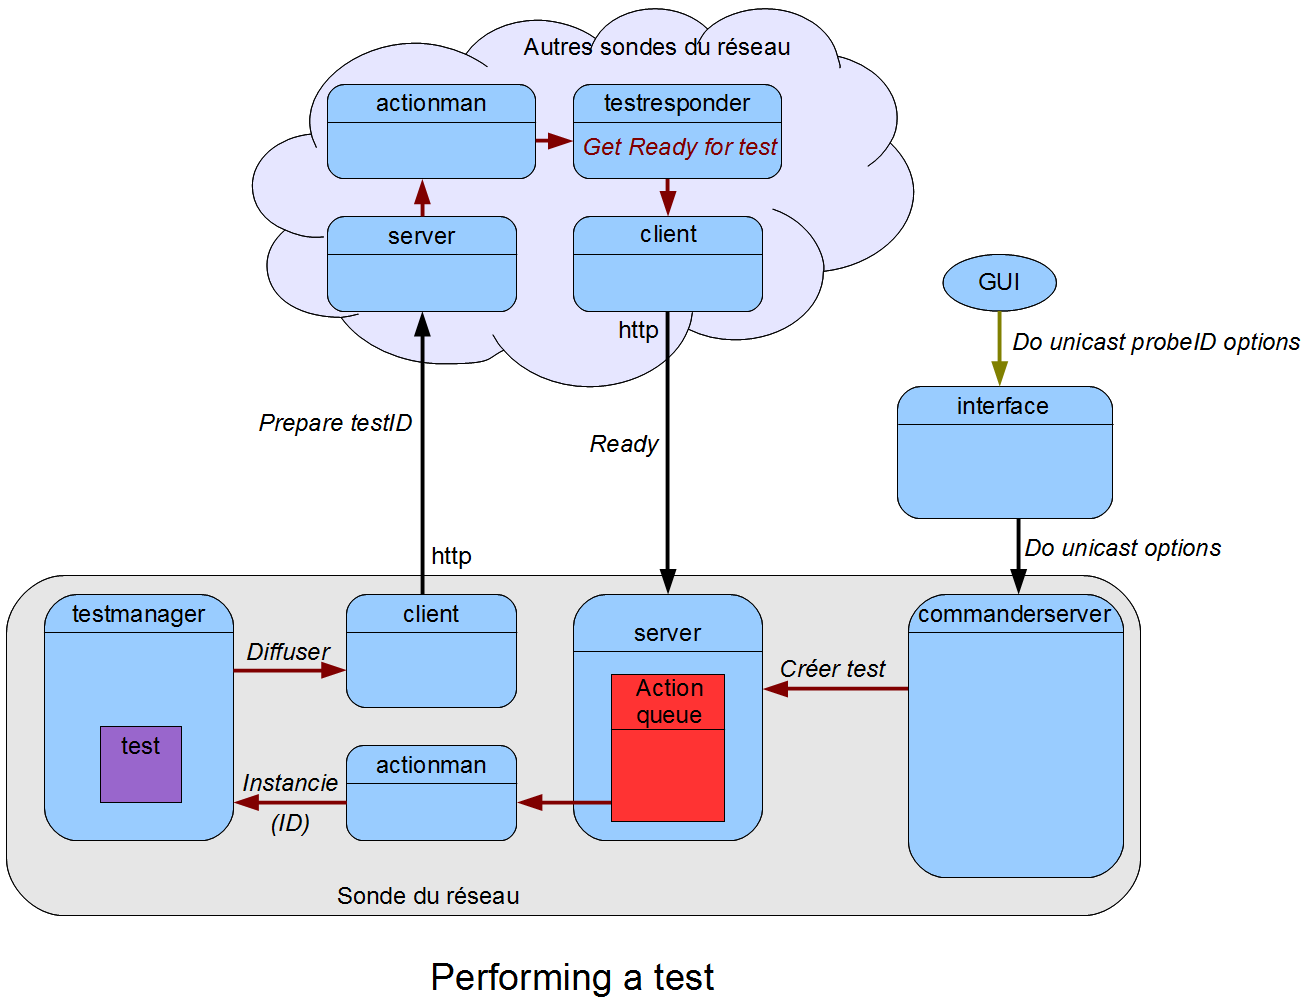
\includegraphics[width=\linewidth]{img/graphTest1.png}
\caption{Exécution d'un test - Etape 1}
\end{figure}

\begin{figure}[!ht]
\centering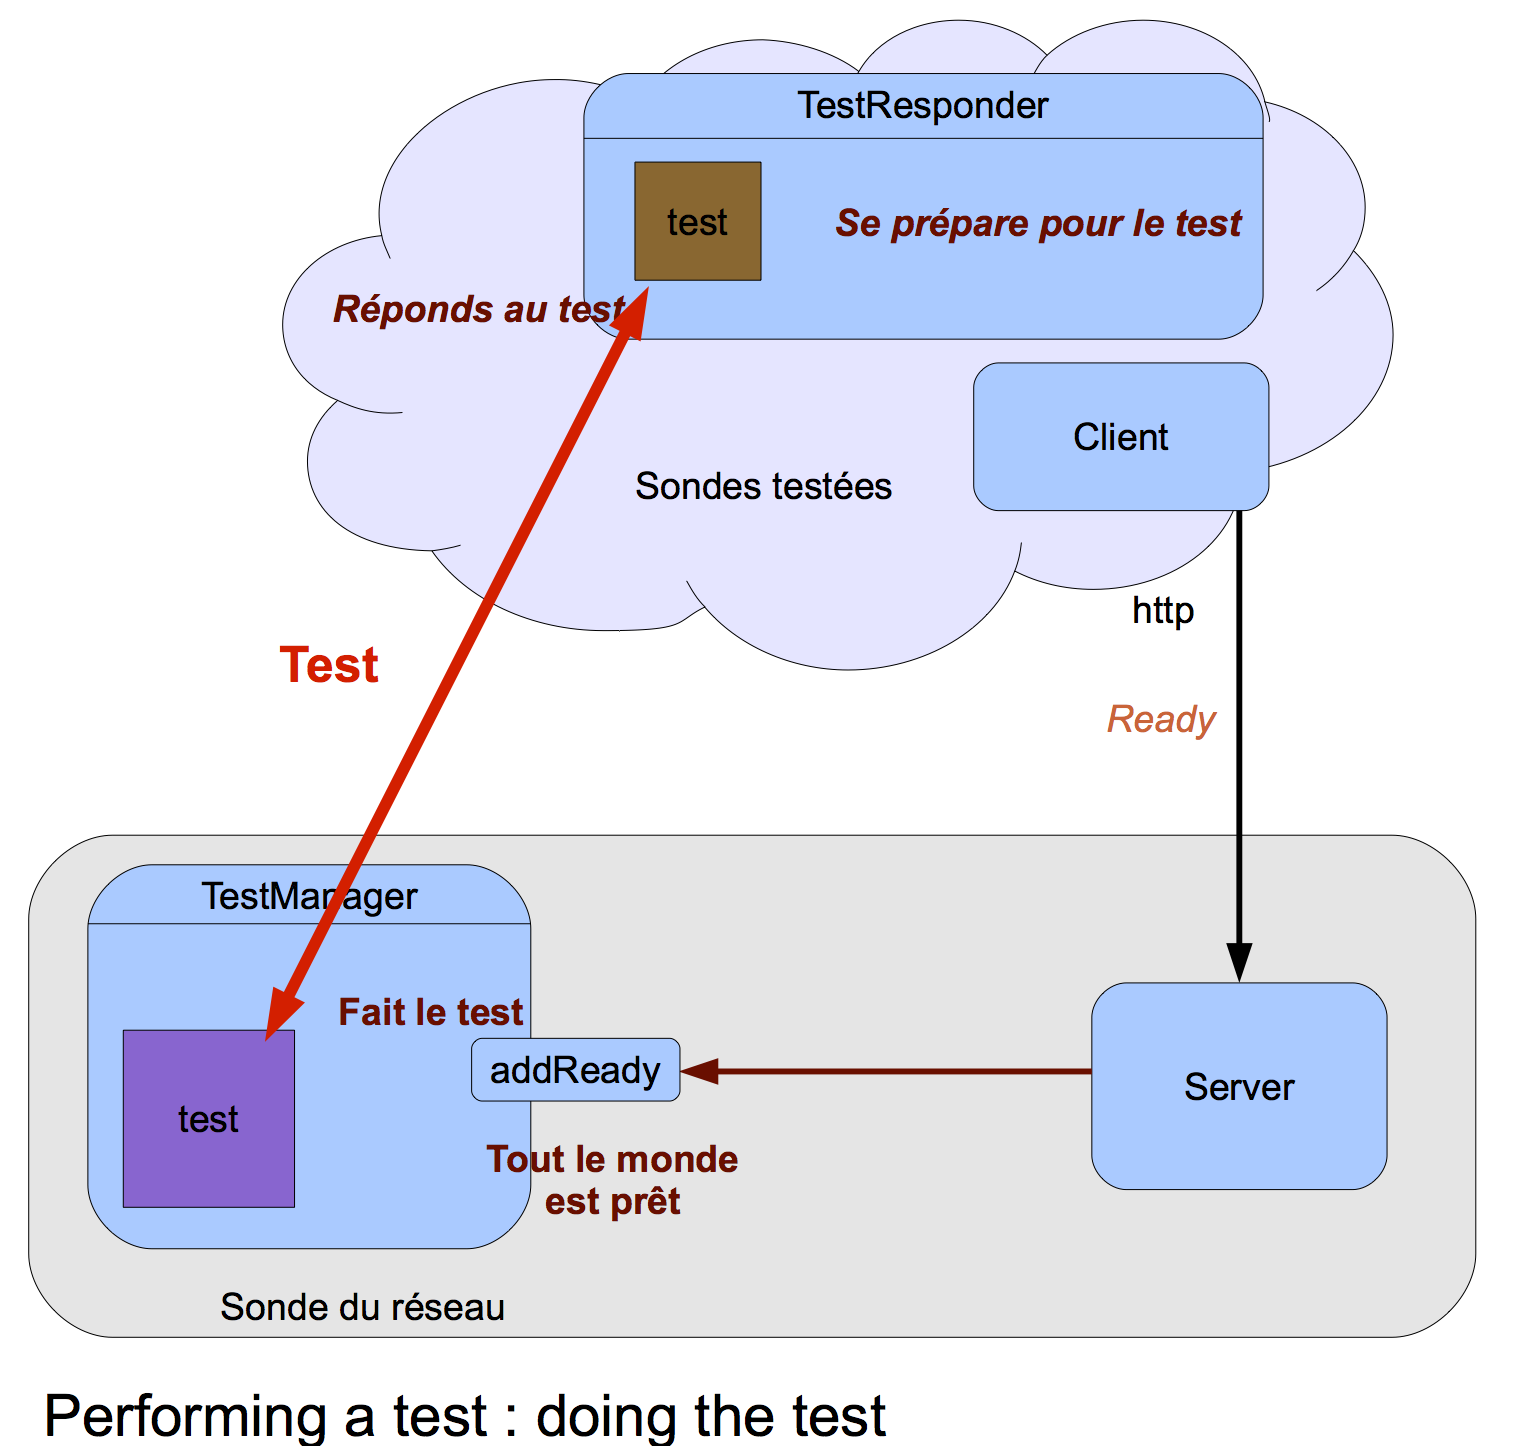
\includegraphics[width=\linewidth]{img/graphTest2.png}
\caption{Exécution d'un test - Etape 2}
\end{figure}

\begin{figure}[!ht]
\centering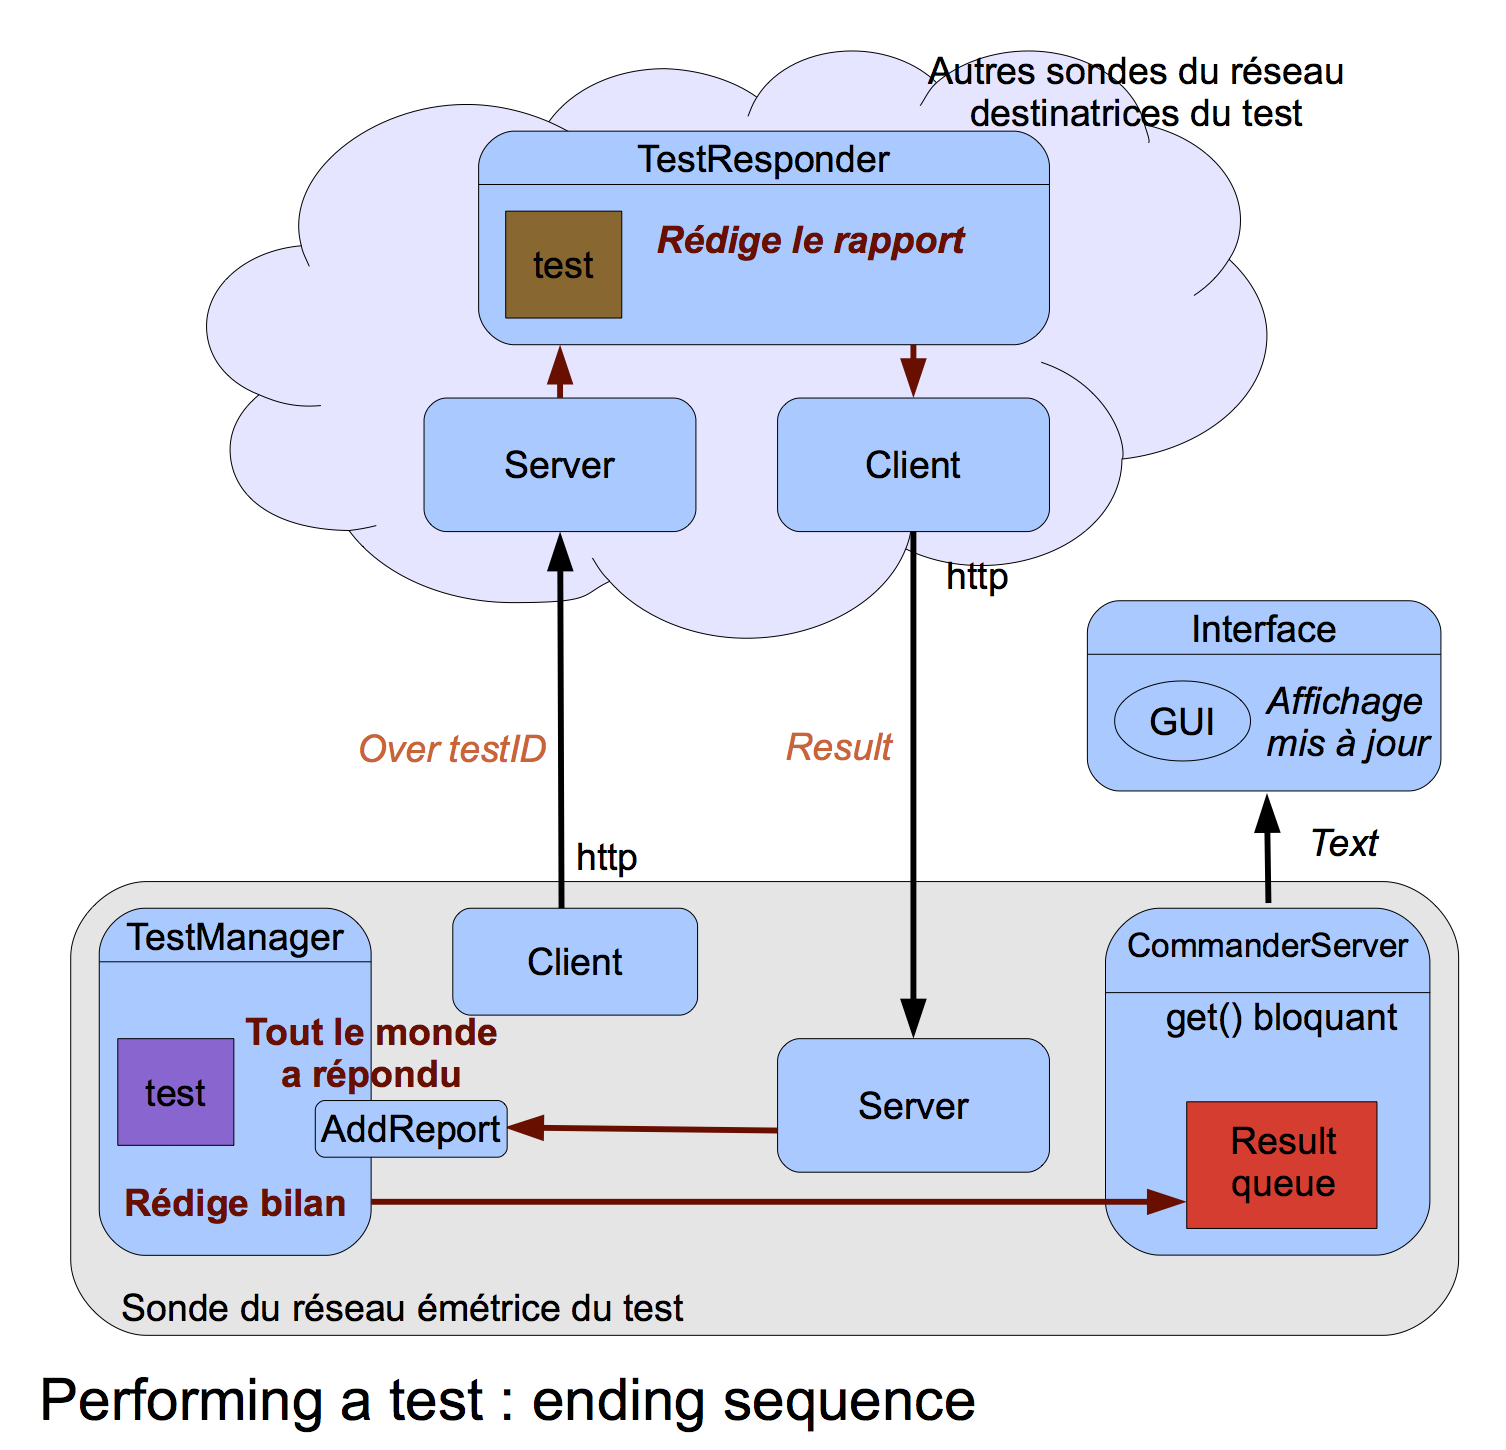
\includegraphics[width=\linewidth]{img/graphTest3.png}
\caption{Exécution d'un test - Etape 3}
\end{figure}

\FloatBarrier

\subsection{Tables de fonctionnement}

\begin{center}
\begin{tabular}{|l|l|c|l|}
\hline
\cd{Server} & \multicolumn{3}{|c|}{\cd{ActionMan}} \\
\hline
\textbf{Message} & \textbf{Action} & & \\
\hline
Add & Add & $\longrightarrow$ & Ajout dans la table / Message "Hello" si nécessaire\\
\hline
Hello & Add & $\longrightarrow$ & Ajout dans la table\\
\hline
\multirow{2}{*}{Bye} & Remove & $\longrightarrow$ & Supprime la sonde de la table\\
\cline{2-4}
 & Quit & $\longrightarrow$ & Diffuse un message "Bye" / Coupe toute les connections sauf la sienne\\
\hline
Prepare & Prepare & $\longrightarrow$ & Lance le test / Bloque jusqu'à la fin du test \\
\hline
\end{tabular}
\end{center}

\begin{center}
\begin{tabular}{|l|l|}
\hline
\multicolumn{2}{|c|}{\cd{CommanderServer}} \\
\hline
\textbf{Message} & \\
\hline
Add & Requête "GET" vers la nouvelle sonde pour connaître son ID / Diffuse un message "Add" \\
\hline
Delete & Envoie un message "Bye"\\
\hline
Do & Met une action "Do" dans le pile d'actions\\
\hline
\end{tabular}
\end{center}

%appendice éventuel
\clearpage
\rhead{Annexe}
\renewcommand{\appendixpagename}{\centering{Annexe : Liste des fonctions Scilab}}
\renewcommand{\labelitemi}{$\bullet$}
\renewcommand{\labelitemiii}{$\cdot$}
\renewcommand{\labelitemii}{$\diamond$}
\renewcommand{\labelitemiv}{$\ast$}
\begin{appendices}
\section{Organisation du code}

\textbf{Thread}
\begin{itemize}
\item \cd{Server}
	\begin{itemize}
	\item \cd{Listener(ThreadingMixIn, HTTPServer, Thread)}
		\begin{itemize}
		\item \cd{RequestHandler(SimpleHTTPRequestHandler)}
		\end{itemize}
	\end{itemize}

\item \cd{CommanderServer}
	\begin{itemize}
	\item \cd{Listener(ThreadingMixIn, HTTPServer, Thread)}
		\begin{itemize}
		\item \cd{RequestHandler(SimpleHTTPRequestHandler)}
		\end{itemize}
	\end{itemize}

\item \cd{Client}
\item \cd{ActionMan}
\end{itemize}



\textbf{Object}
\begin{itemize}
\item \cd{Message} 
	\begin{itemize}
	\item \cd{Add}
	\item \cd{Hello}
	\item \cd{Bye}
	\item \cd{TestMessage}
	\begin{itemize}
		\item \cd{Prepare}
		\item \cd{TesterMessage}
			\begin{itemize}
			\item \cd{Over}
			\item \cd{Abort}
			\end{itemize}
		\item \cd{TesteeMessage}
			\begin{itemize}
			\item \cd{Ready}
			\item \cd{Result}
			\end{itemize}
		\end{itemize}
	\end{itemize}

\item \cd{Action} 
	\begin{itemize}
	\item \cd{Add}
	\item \cd{Remove}
	\item \cd{Do}
	\item \cd{Prepare}
	\item \cd{Quit}
	\end{itemize}

\item \cd{Test}
	\begin{itemize}
	\item \cd{Unicast}
	\item \cd{Multicast}
	\item \cd{Broadcast}
	\item \cd{Empty}
	\end{itemize}

\item \cd{TestManager}
\item \cd{TestResponder}

\item \cd{Interface}
	\begin{itemize}
	\item \cd{Gui}
	\item \cd{Cli}
	\end{itemize}
\item \cd{Parser}

\item \cd{Probe}
\item \cd{ProbeStorage}
\item \cd{Consts}
\item \cd{Params}
\item \cd{Identification}

\item \cd{Exception}
	\begin{itemize}
	\item \cd{NoSuchProbe}
	\item \cd{TestInProgress}
	\item \cd{NoSuchCommand}
	\end{itemize}
\end{itemize}
\end{appendices}
\end{document}
